\documentclass[a4paper,9pt,twocolumn]{ltjsarticle} % ← lualatex ではなく ltjsarticle
\usepackage[ipaex]{luatexja-preset}  % 日本語フォントの手当て(IPAex)
\usepackage{ifthen}
\usepackage{algorithm}
\usepackage{algorithmicx}
\usepackage{algpseudocode}
\usepackage{amsmath}
\usepackage{graphicx}
\usepackage{here}

\makeatletter
\renewcommand{\maketitle}{%
\ifthenelse{\equal{\course}{bachelor}}{%
  \begin{titlepage}
    \vspace*{10mm}
    \begin{center}
      {\huge\@gyear 年度\hspace{5mm}\@thesis\par}
      \vfill
      {\huge\bfseries\@title\par}
      \vfill
      \vspace{10mm}
      {\Large\@date\par}
      \vspace{20mm}
      {\Large\@department\@departmentsfx\par}
      {\Large (学生番号: \@studentid)\par}
      \vspace{5mm}
      {\LARGE\@author\par}
      \vspace{55mm}
      {\Large 和歌山大学\@faculty}
      \vspace{10mm}
    \end{center}
  \end{titlepage}}{}%
\ifthenelse{\equal{\course}{master}}{%
  \begin{titlepage}
    \begin{center}
      \vspace*{8mm}
      {\Large\@gyear 年度\hspace{5mm}\@thesis\par}
      \vfill
      {\huge\bfseries\@title\par}
      \vfill
      {\Large \@date\par}
      \vspace{40mm}
      {\Large 和歌山大学\@faculty\par}
      \vspace{27mm}
      {\Large 学生番号: \@studentid\par}
      {\LARGE \@author\par}
      \vspace*{28mm}
    \end{center}
  \end{titlepage}%
  \begin{titlepage}
    \begin{center}
      \vspace*{8mm}
      {\huge\@etitle\par}
      \vspace{12mm}
      {\Large by\par}
      \vspace{9mm}
      {\huge\@eauthor\par}
      \vspace{27mm}
      {\LARGE\@ethesis\par}
      \vfill
      {\Large \@efaculty\par}
      \vspace{4mm}
      {\Large Wakayama University\par}
      \vspace{23mm}
      {\Large \@edate\par}
      \vspace*{14mm}
    \end{center}
  \end{titlepage}}{}%
}

%% 概要
\def\abstract{\newpage\pagenumbering{roman}\section*{概 要}}
\def\endabstract{}
%% 目次
\def\tableofcontents{%
  \newpage
  \section*{目 次\@mkboth{目 次}{目 次}}
  \@starttoc{toc}}
%% 図目次
\def\listoffigures{%
  \newpage
  \section*{図 目 次\@mkboth{図 目 次}{図 目 次}}
  \@starttoc{lof}}
%% 表目次
\def\listoftables{%
  \newpage
  \section*{表 目 次\@mkboth{表 目 次}{表 目 次}}
  \@starttoc{lot}}
%% 謝辞
\def\acknowledgements{\newpage\section*{謝 辞}}
\def\endacknowledgements{}
%% 参考文献
\def\thebibliography#1{%
  \newpage
  \section*{参 考 文 献\@mkboth{参 考 文 献}{参 考 文 献}}
  \list{[\arabic{enumi}]}
    {\settowidth{\labelwidth}{[#1]}
     \leftmargin=\labelwidth
     \advance\leftmargin by \labelsep
     \usecounter{enumi}}
  \def\newblock{\hskip .11em plus .33em minus .07em}
  \sloppy
  \clubpenalty=4000 \widowpenalty=4000
  \sfcode`\.=1000\relax}
\let\endthebibliography=\endlist
\makeatother

\makeatletter
\def\course{bachelor}
\def\@gyear{2025}
\def\@thesis{卒業論文}
\def\@title{DIDに基づいたIoTデータ管理システムの構築と評価}
\def\@date{2026年2月10日}
\def\@department{システム工学部}
\def\@departmentsfx{システム工学科}
\def\@studentid{60276128}
\def\@author{竹内 結哉}
\def\@faculty{システム工学部}
\makeatother

\begin{document}
\maketitle

\section{はじめに}
近年,IoT機器の爆発的な増加に伴い,生成されるデータ量は急激に増加している.
さらに,IoTは家庭や産業,医療,農業など多様な分野で活用されるようになり,生成されるデータの種類や粒度も一層多様化している.

しかし,従来の中央集権型によるIoTデータ管理には,以下の3つの課題が存在する.
第一に,スケーラビリティの問題である.IoTデバイスの急増により,中央サーバーへの負荷が指数関数的に増大し,処理能力の限界に達する可能性がある.
第二に,セキュリティ上の問題である.中央サーバーは単一障害点となりやすく,攻撃対象として脆弱である.
第三に,プライバシー保護の問題である.個人情報を含むIoTデータが集中することで,情報漏洩時の被害が甚大化するリスクがある.

これらの課題を解決するために,本研究ではユーザー主権型IDに基づいた分散型データ管理システムの実現を目指す.
本システムは,以下の三点を重視して設計されている.

\begin{enumerate}
\item データの分散管理:中央集権型から脱却し,分散型ファイルシステムであるInterPlanetary File System(以下IPFS)を用いることで,
      単一障害点を排除しシステムの堅牢性を向上させる.
\item ユーザーの真正性確保:分散管理環境におけるなりすまし防止のため,分散型識別子であるDecentralized Identity(以下DID)を活用し,
      データ所有者の身元を保証する.
\item データの信頼性と改ざん防止:ブロックチェーンを活用し,データが改ざんされていないことを検証可能とする.
\end{enumerate}

以上の要素を組み合わせることで,IoTデータに対する分散型かつ信頼可能な管理基盤を構築することを目指す.

\section{関連研究}
IoTデータ管理の分散化に関する研究として,先行研究\cite{cite1}がある.

\section{準備}
本研究では,分散型データ管理の基盤技術としてIPFS,DID,およびブロックチェーンを用いる.
本章では,これらの技術の概要を説明し,さらに本研究で使用した実験環境について述べる.

\subsection{IPFS}
IPFSは,分散型のファイルシステムであり,コンテンツ指向のアドレッシング方式を採用している.
従来のURLが「場所」に基づいてデータを参照するのに対し,IPFSではデータ内容から生成されるハッシュ値を用いて「内容」を参照する.
これにより,同一のデータは同一のハッシュ値で一意に識別され,データの改ざん検知が容易になるとともに,
ネットワーク上の複数ノードに分散保存することで耐障害性を高めることができる.
本研究では,IPFSの実装として\texttt{go-ipfs}を用いた.
これはIPFSの公式実装であり,Go言語で開発されている.

\subsection{DID}
DIDは,自己主権型アイデンティティを実現するための分散型識別子である.
従来のインターネットにおける認証・識別は,中央集権的な認証局やサービス提供者に依存していたため,
単一障害点や利用者のプライバシー保護に課題があった.
これに対しDIDは,ユーザー自身が管理可能な識別子を提供することで,第三者に依存せずに真正性を保証できる仕組みを実現する.
DID Documentと呼ばれる文書には公開鍵やサービスエンドポイントなどが含まれ,これにより利用者の認証やデータ検証を行うことができる.

\subsection{ブロックチェーン}
ブロックチェーンは,分散型台帳技術の一種であり,取引情報をブロックとして記録し,チェーン上に連結することで,
データの改ざん耐性を保証する.
各ブロックは暗号学的ハッシュにより前後のブロックと結合されており,一部のデータが改ざんされると以降のブロックすべてが不整合となるため,
改ざん検知が容易である.
また,ネットワークに参加する複数ノード間で合意形成を行い,信頼できる台帳を分散的に維持する仕組みを持つ.
本研究では実験環境としてEthereum互換のローカルブロックチェーン環境である\texttt{Ganache}を使用した.
Ganacheは開発用に特化したブロックチェーンシミュレータであり,高速なテスト実行やトランザクションの記録確認を容易に行うことができる.

\section{システム構成}

\subsection{全体像}
本研究で提案するシステムの全体像を図\ref{fig:system-overview}に示す.

\begin{figure}[H]
  \centering
  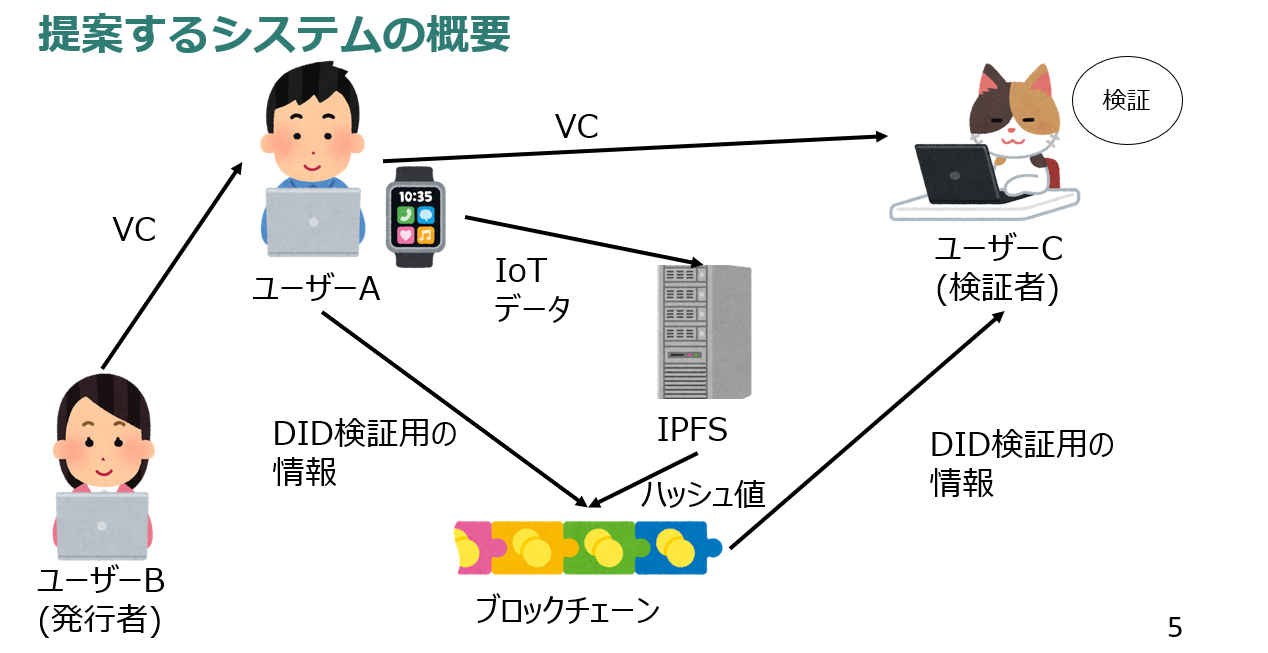
\includegraphics[width=0.9\linewidth]{figure1.png}
  \caption{提案システムの全体像}
  \label{fig:system-overview}
\end{figure}

\section{実験と考察}

\section{まとめ}

\bibliographystyle{junsrt}
\bibliography{references}
\end{document}
